\documentclass[a4paper,11pt]{article}

\usepackage[utf8]{inputenc}
%\usepackage[ngerman]{babel}
\usepackage{microtype,ellipsis,fixltx2e,mparhack,graphicx,url}
\usepackage[pdftex,bookmarks=true,hypertexnames=false,bookmarksnumbered=true]{hyperref}
\usepackage{textcomp}
\usepackage{vmargin}
% \usepackage[scaled=0.9]{helvet}
\usepackage{longtable}
% \normalfont % in case the EC fonts aren't available
% \fontfamily{helvetica}
%\numberwithin{equation}{section}
% \renewcommand*\familydefault{\sfdefault}

\usepackage{tikz}
\usetikzlibrary{shapes,arrows}
% Define block styles
% \tikzstyle{decision} = [diamond, draw, fill=blue!20, text width=4.5em, text badly centered, node distance=3cm, inner sep=0pt]
\tikzstyle{block} = [rectangle, draw, text width=6em, text centered, rounded corners, minimum height=4em]
\tikzstyle{line} = [draw, -latex']
% \tikzstyle{cloud} = [draw, ellipse,fill=red!20, node distance=3cm, minimum height=2em]

\usepackage{cite}
\bibliographystyle{unsrt}

% amsmath package, useful for mathematical formulas
\usepackage{amsmath}

% amssymb package, useful for mathematical symbols
\usepackage{amssymb}



\begin{document}


\vspace{5cm} 
    \huge
    \textbf{[CHA-LEARN] Reconstruction of synaptic network topology from calcium fluorescence signals}
    \normalsize
%\vspace{5cm}

\vspace{1cm}
(This file is work in progress. Olav Stetter, \today)
\vspace{1cm}


\section{About this package}

This package is designed to be used as a starting point for working on the network reconstruction challenge of the CHA-LEARN (Challenges in Machine Learning) initiative.
A number of example data sets of network topologies and simulated calcium fluorescence data is provided, as well as scripts to generate new data sets.

The general idea is to reconstruct, from an observed time series of neuronal activity (in this case calcium fluorescence signals), the synaptic connectivity network underlying the dynamics.

For simplicity, we limit this challenge to simulation of purely excitatory networks \emph{in vitro}, so in a situation where all neurons are experimentally accessible.
For an overview about these systems, see~\cite{Eckmann:2007p48}.
An important characteristic feature of these networks is ``bursting'', spontaneous synchronization events that excite the entire network for a period of about 200ms~\cite{Eytan:2006p66,Cohen:2008cv}, which likely need to be taken into account when approaching the challenge.


\section{Dependencies}

If you want to compare a given reconstruction methods with GTE, there is a set of simulations and reconstruction results included in this package for network sizes $N = 50, 100 \text{ and } 500$ and clustering indices of $CC = 0.1, 0.2, 0.3, 0.4, 0.5 \text{ and } 0.6$.
(Note that by ``clustering index'', we mean the population average of the full clustering index as defined in~\cite{Fagiolo:2007p53}.)
The network topologies are given in YAML format, and the simulated fluorescence time series and the resulting ROC curves are included both in standard CSV format. As such, there are no dependencies.

If however, you would like to create new topologies, simulate new spike data or fluorescence and evaluate those, you will need to have the following software installed:

\begin{itemize}
  \item Mathematica
  \item NEST, for simulating the leaky integrate-and-fire model~\cite{Gewaltig:NEST}
  \item TE-Causality, the software that was used to generate the GTE reconstructions
\end{itemize}


\section{How to generate reconstructions in the GTE framework}

The steps to go from scratch to the final reconstruction are shown in Figure~\ref{fig:flow_chart_1}. Each of them is described in detail in the sections below.

\begin{figure}
  \begin{center}
    %!TEX root = /Users/olav/Desktop/Doktorarbeit/Causality/challenge/documentation/CHA-readme.tex

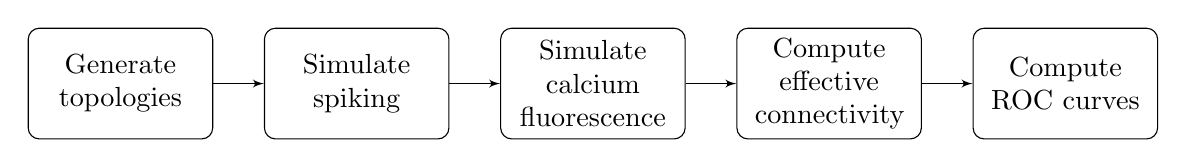
\begin{tikzpicture}[node distance = 3cm, auto]
  % Place nodes
  \node [block] (topos) {Generate topologies};
  \node [block, right of=topos] (spikes) {Simulate spiking};
  \node [block, right of=spikes] (fluoro) {Simulate calcium fluorescence};
  \node [block, right of=fluoro] (rec) {Compute effective connectivity};
  \node [block, right of=rec] (rocs) {Compute ROC curves};
  % \node [block, below of=identify] (evaluate) {evaluate candidate models};
  % \node [block, left of=evaluate, node distance=3cm] (update) {update model};
  % \node [decision, below of=evaluate] (decide) {is best candidate better?};
  % \node [block, below of=decide, node distance=3cm] (stop) {stop};
  % Draw edges
  \path [line] (topos) -- (spikes);
  \path [line] (spikes) -- (fluoro);
  \path [line] (fluoro) -- (rec);
  \path [line] (rec) -- (rocs);
  % \path [line] (identify) -- (evaluate);
  % \path [line] (evaluate) -- (decide);
  % \path [line] (decide) -| node [near start] {yes} (update);
  % \path [line] (update) |- (identify);
  % \path [line] (decide) -- node {no}(stop);
  % \path [line,dashed] (expert) -- (init);
  % \path [line,dashed] (system) -- (init);
  % \path [line,dashed] (system) |- (evaluate);
\end{tikzpicture}

  \end{center}
  \caption{Procedure to generate reconstructions using the included scripts.}
  \label{fig:flow_chart_1}
\end{figure}


\subsection{Generating topologies}

Using the Mathematica script in \emph{CHA-generate\_topology.nb} network topologies of arbitrary size and from one of two ensembles can be generated:
\begin{itemize}
  \item Networks where the probability of connection depends on the distance between two nodes using a Gaussian kernel (the ``local ensemble''), and
  \item networks that are characterized instead by an average clustering coefficient (the ``non-local clustering ensemble'').
\end{itemize}

Note that both of these ensembles include the random graph as a limiting case, either for the length scale of the connectivity kernel going to infinity, or with a clustering coefficient that is equal to the overall probability of connection.

\begin{table}[ht]
  % [!ht]
  \begin{center}
    \begin{tabular}
      {|ll|l|} %\hline Parameter & value \\ 
      \hline
      $N$ & network size & 50, 100, 500 \\
      $CC$ & target clustering coefficient & 0.1, 0.2, 0.3, 0.4, 0.5, 0.6 \\
      $l$ & length of square of simulated network & 1.0mm \\
      $d_{\text{min}}$ & minimum distance between neurons & 0.01mm \\
      \hline
    \end{tabular}
  \end{center}
  \caption{List of parameters used in the simulation of network topologies.}
  \label{tab:parameters_topos}
\end{table}


\subsection{Simulate spiking activity}

For simulating the leaky integrate-and-fire neurons with depressive synapses~\cite{Tsodyks:1997p5532,Tsodyks:2000p3237} we use the NEST (Neural Simulation Technology, see~\cite{Gewaltig:NEST}) script that is included in \emph{CHA-adaptive-bursts.py}.
The parameters used are listed in Table~\ref{tab:parameters_spiking}.

Here we assume that each neuron receives independent Poisson inputs either from the outside or due to internal thermal fluctuations, called ``external'' inputs, and from other neurons that are connected to it, called ``internal'' inputs.
Using an iterative procedure, the NEST simulator will find the synaptic weight of internal connections that yields a biologically realistic bursting rate.

\begin{table}[ht]
  % [!ht]
  \begin{center}
    \begin{tabular}
      {|ll|l|} %\hline Parameter & value \\ 
      \hline
      $C_m$ & membrane capacitance of neurons & 1.0pF \\
      $\tau_m$ & membrane time constant & 20ms \\
      $\tau_{\text{ref}}$ & refractory time & 2.0ms \\
      $E_L$ & resting voltage (also voltage after reset) & -70mV \\
      $V_{\text{th}}$ & voltage threshold & -50mV \\
      $\delta$ & synaptic delay & 2.0ms \\
      $\tau_{\text{rec}}$ & recovery time constant of depressive synapses & 500ms \\
      $\tau_{\text{fac}}$ & time constant of depressive synapses for facilitation & 0ms \\
      $U$ & fraction of neurotransmitters used upon spiking & 0.3 \\
      $f_{\text{burst}}$ & target bursting rate & 0.1Hz \\
      $\Delta f_{\text{burst}}$ & accuracy goal of target bursting rate & 0.01Hz \\
      $\nu_{\text{ext}}$ & rate of external inputs & 0.2Hz \\
      $J_{\text{ext}}$ & synaptic weight of external inputs & 11.2pA \\
      $J_{\text{int}}^0$ & initial value of synaptic weight of internal synapses & 8.0pA \\
      $T_{\text{adapt}}$ & simulation time for adaptation phase & 200s \\
      $T$ & simulation time (for actual simulation) & 3600s \\
      \hline
    \end{tabular}
  \end{center}
  \caption{List of parameters used in the simulation of neuronal spiking activity.}
  \label{tab:parameters_spiking}
\end{table}



\subsection{Simulate fluorescence imaging}

To simulate the calcium fluorescence time series, we use a standard model from the literature~\cite{Vogelstein:2009p3029,Mishchencko:2009p4301} and the script \emph{CHA-simulate\_fluorescence.nb}.
The parameters are listed in Table~\ref{tab:parameters_fluoro}.

Note that the package that computes the causality measures later, TE-Causality, is able to simulate fluorescence in the same way by itself, so this step can be skipped and is only included here for using the fluorescence time series with other methods for comparison.

\begin{table}[ht]
  % [!ht]
  \begin{center}
    \begin{tabular}
      {|ll|l|} %\hline Parameter & value \\ 
      \hline
      $\tau_F$ & decay time of calcium fluorescence & 1.0s \\
      $A_{\text{Ca}}$ & change in bound calcium concentration upon spiking & 50 $\mu$Mol \\
      $K_d$ & saturation level of the bound calcium concentration & 300 $\mu$Mol \\
      $n_{\text{sat}}$ & order of saturating Hill function & 1 \\
      $\sigma_{\text{noise}}$ & standard deviation of camera noise & 0.03 \\
      $\sigma_{\text{sc}}$ & light scattering width & 0.5mm / $\sqrt{N}$ \\
      $A_{\text{sc}}$ & light scattering amplitude & 0.15 \\
      $\tau_F$ & length of an image frame & 20ms \\
      \hline
    \end{tabular}
  \end{center}
  \caption{List of parameters used in the simulation of the calcium fluorescence signal.}
  \label{tab:parameters_fluoro}
\end{table}


\subsection{Calculate GTE}

In this reference implementation, the reconstruction of the effective connectivity network is generated using a causal measure called Generalized Transfer Entropy~(GTE)~\cite{Stetter:2012vt,Orlandi:2013uz}, an extension of Transfer Entropy as introduced in~\cite{Schreiber:2000p79}.
We use the implementation of the the TE-Causality package (see \emph{http://www.network-reconstruction.org/}) and the corresponding control file in \emph{reconstructions/control.txt}.
The parameters are listed in Table~\ref{tab:parameters_rec}.

Please see the GitHub repository for documentation on how to install or use this package.

\begin{table}[ht]
  % [!ht]
  \begin{center}
    \begin{tabular}
      {|ll|l|} %\hline Parameter & value \\ 
      \hline
      $b$ & number of bins used for estimating probability distributions & 2 \\
      $k$ & assumed Markov order & 2 \\
      $x_{\text{sep}}$ & value of the difference signal of fluorescence used to separate the bins & 0.12 \\
      $\tilde{g}$ & conditioning level & 0.3 \\
      \hline
    \end{tabular}
  \end{center}
  \caption{List of parameters used in the computation of GTE.}
  \label{tab:parameters_rec}
\end{table}


\subsection{Compute ROC curves}

Finally, the quality of reconstruction is quantified in \emph{CHA-analyze\_reconstruction.nb}.
Typically, the reconstruction performance is assed by the fraction of true positives achieved at a fraction of 10\% of false positives.



\section{Copyright}

All of the files in this package can be copied, modified, used for commercial or non-commercial purpose, as long as you keep the following copyright message in the source files:

This program is free software: you can redistribute it and/or modify it under the terms of the GNU General Public License as published by the Free Software Foundation, either version 3 of the License, or (at your option) any later version.
This program is distributed in the hope that it will be useful, but WITHOUT ANY WARRANTY; without even the implied warranty of MERCHANTABILITY or FITNESS FOR A PARTICULAR PURPOSE.  See the GNU General Public License for more details.

You should have received a copy of the GNU General Public License along with this program.  If not, see \emph{http://www.gnu.org/licenses/}.



% \clearpage
\bibliography{references}


\end{document}
